\documentclass[english]{article}

\setlength{\parskip}{\smallskipamount}

\setlength{\parindent}{0pt}

\usepackage[T1]{fontenc}

\usepackage[latin9]{inputenc}

\usepackage{geometry}

\geometry{verbose,tmargin=1in,bmargin=1cm,lmargin=2cm,rmargin=2cm}

\usepackage{graphicx}

\usepackage{booktabs}

\makeatletter

\newcommand{\testDocOne}{T_1}
\newcommand{\testDocTwo}{T_2}

\newcommand{\testOne}{1}

\newcommand{\testTwo}{2}

\usepackage{siunitx}

\makeatother

\begin{document}

\section{Level 1 header}

This is the document body.

Testing preamble constants: $\testOne$ and $\testTwo$.

Testing included file: $\testDocOne$ and $\testDocTwo$.

\subsection{Included graphics}

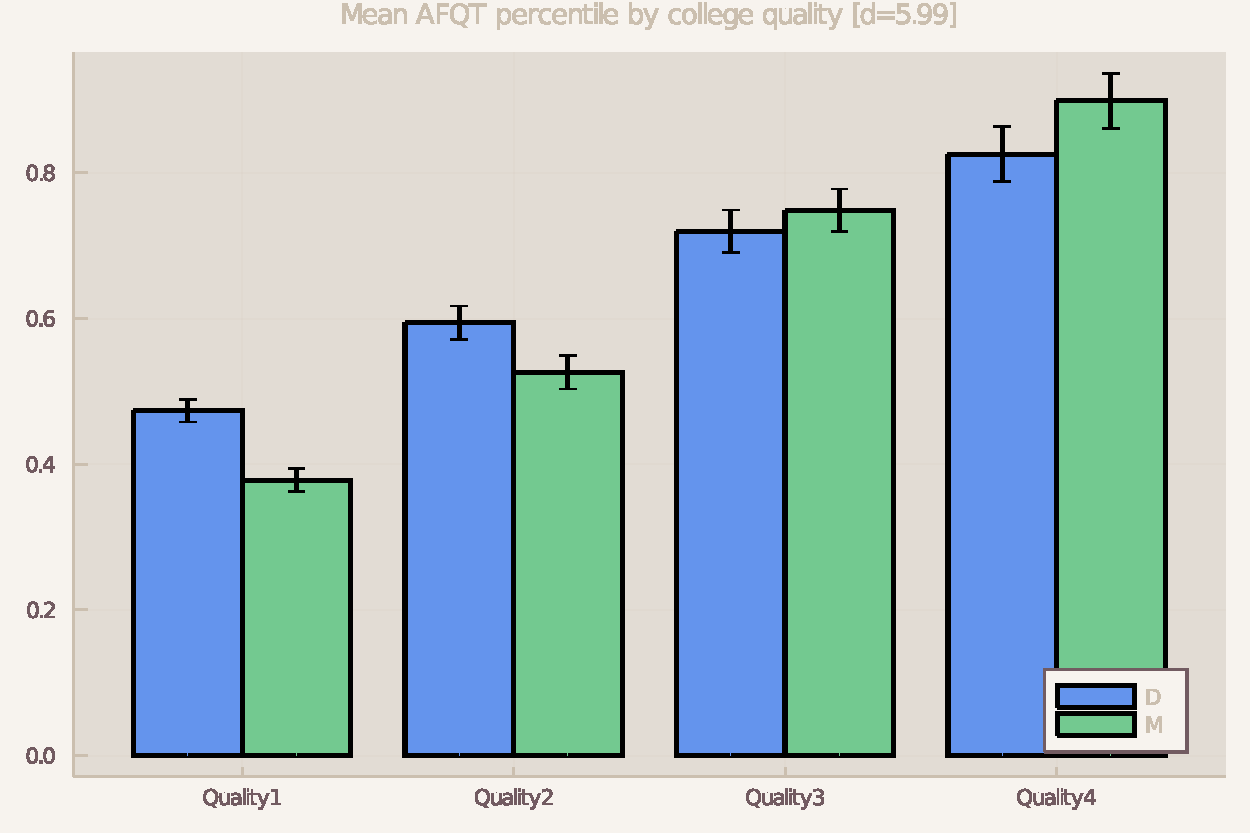
\includegraphics[width=0.75\textwidth]{/Users/lutz/Documents/julia/LatexLH/test/test_files/afqtMeanByQual.pdf}

afqtMeanByQual.pdf

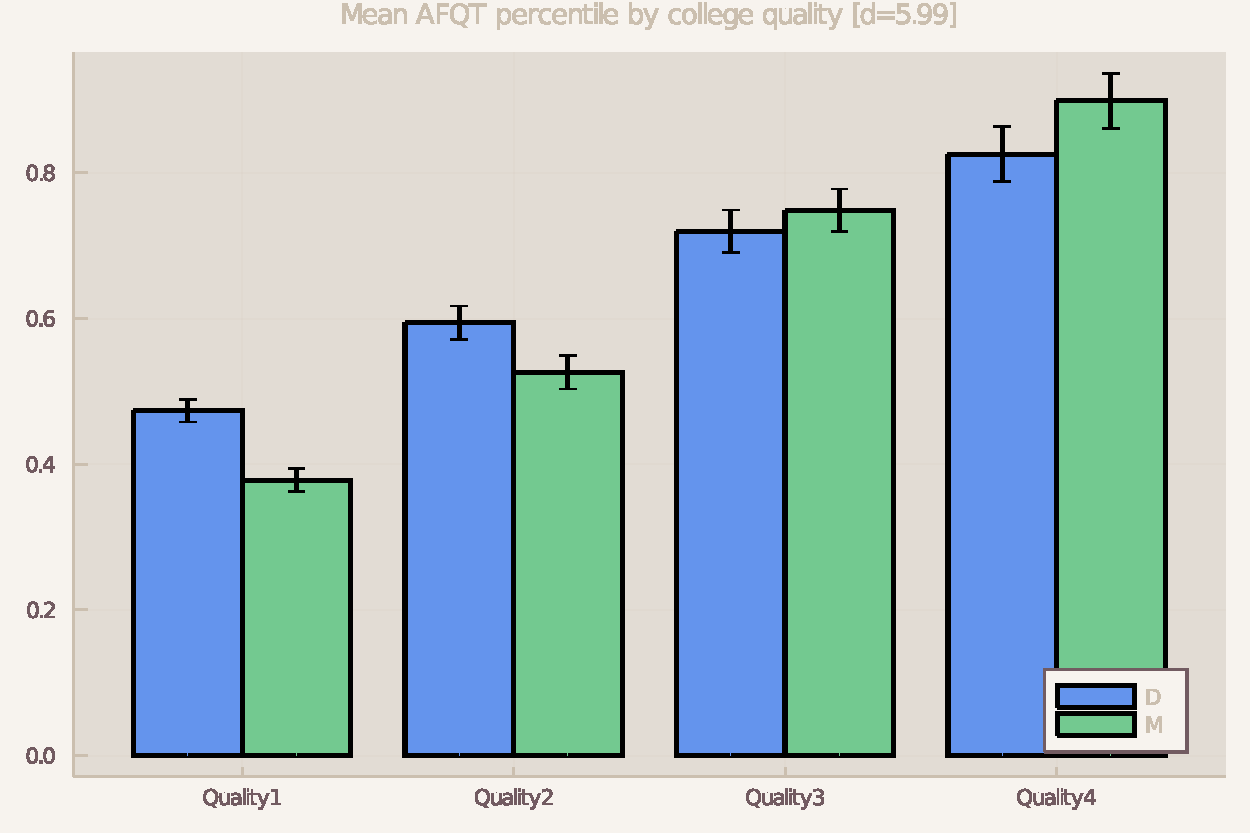
\includegraphics[width=0.5\textwidth]{/Users/lutz/Documents/julia/LatexLH/test/test_files/afqtMeanByQual.pdf} 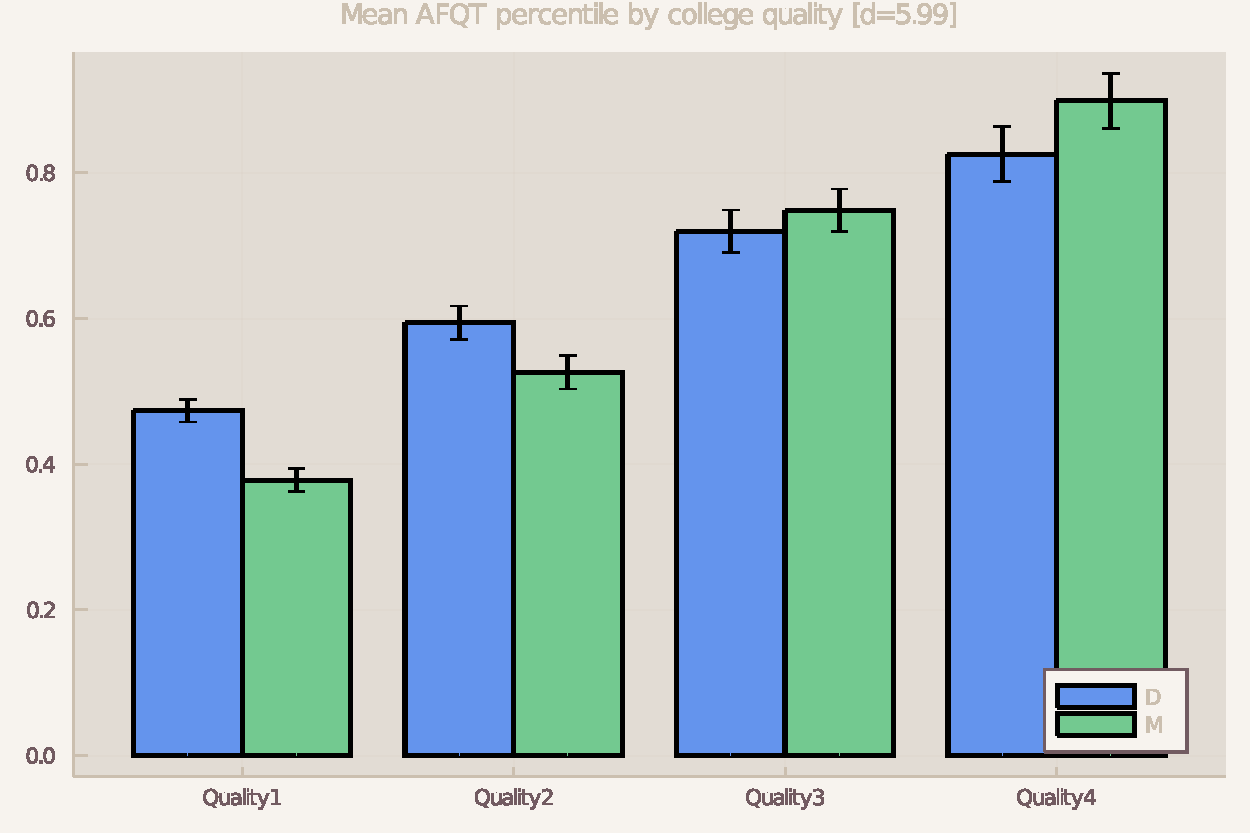
\includegraphics[width=0.5\textwidth]{/Users/lutz/Documents/julia/LatexLH/test/test_files/afqtMeanByQual.pdf}

fracGradByQual.pdf

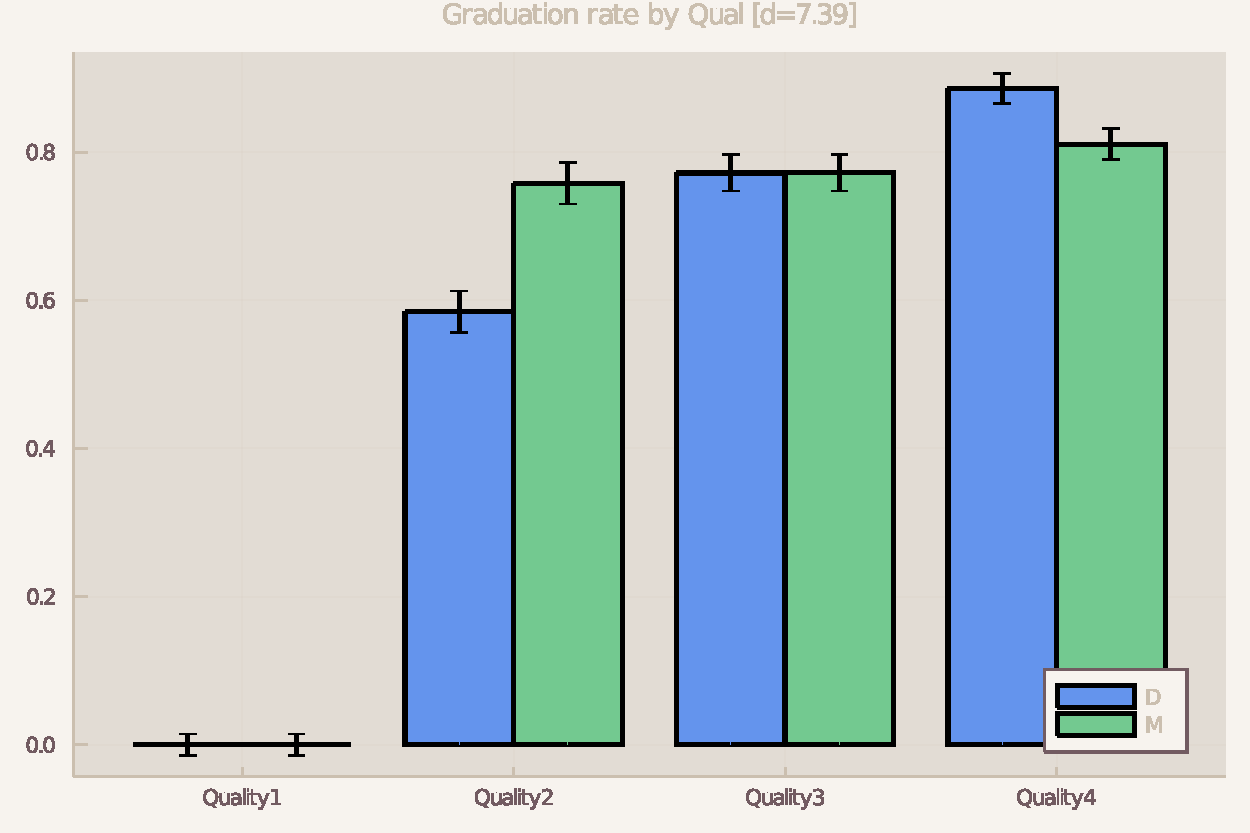
\includegraphics[width=0.5\textwidth]{/Users/lutz/Documents/julia/LatexLH/test/test_files/fracGradByQual.pdf} 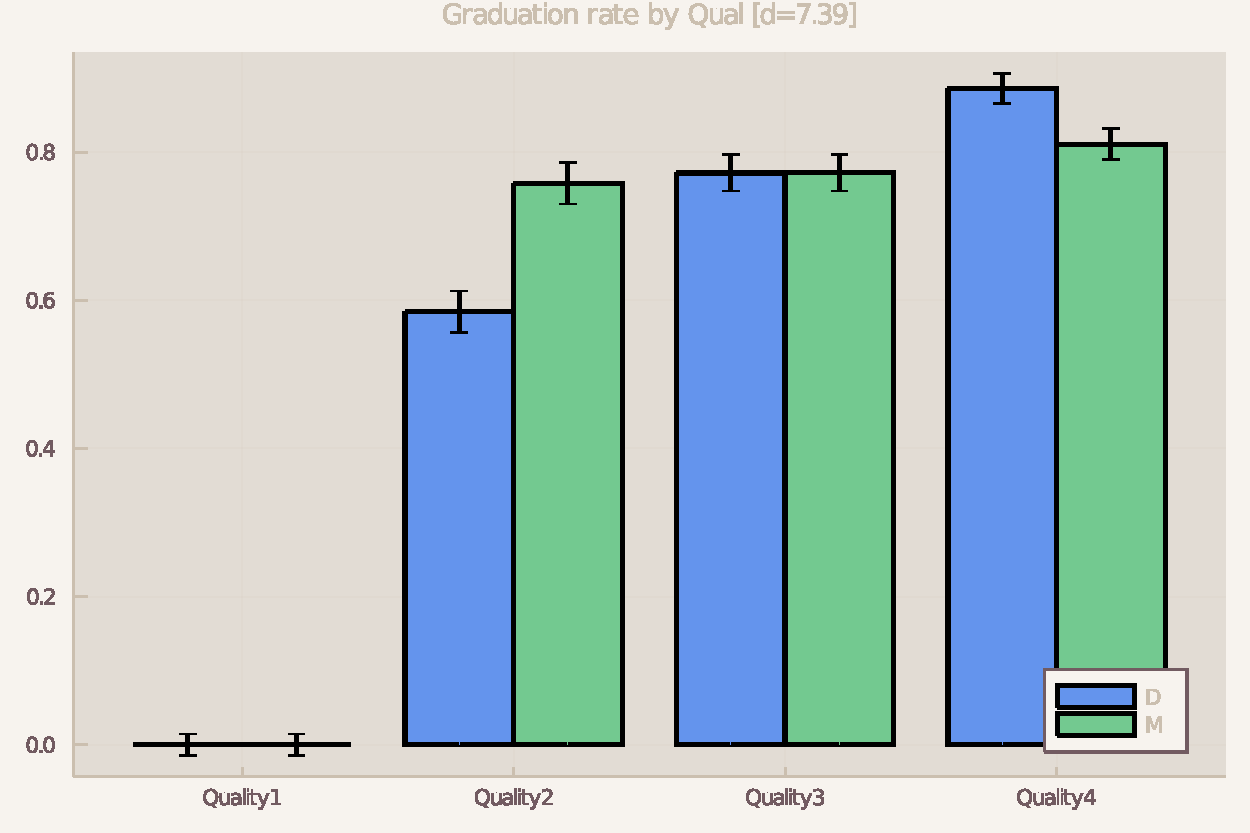
\includegraphics[width=0.5\textwidth]{/Users/lutz/Documents/julia/LatexLH/test/test_files/fracGradByQual.pdf}

\subsection{Included tables}

\begin{tabular}{lSSSS} 
\toprule 
 & \multicolumn{3}{c}{Heading 1} &  \\ 
cell1 & \multicolumn{4}{c}{cell2} \\ 
\cline{2-5} 
x1 & 1.2 & 2.3 & 3.4 & 4.5 \\ 
\bottomrule 
\end{tabular} 


\end{document}

